\documentclass[11pt]{article}

\usepackage[utf8]{inputenc}

\usepackage{amsmath,amssymb,booktabs,tabularx,array,longtable}
\usepackage{graphicx,microtype,float}
\usepackage[a4paper,margin=24mm]{geometry}
\usepackage[hidelinks]{hyperref}
\usepackage{url}
\usepackage[numbers,sort&compress]{natbib}
\setlength{\emergencystretch}{2em}
\setlength{\parskip}{3pt}
\newcommand{\FloatBarrier}{\par}
\newcommand{\ind}{\mathbf{1}}
\newcommand{\R}{\mathbb{R}}
\newcommand{\pos}[1]{\left(#1\right)_{+}}
\newcommand{\clip}{\operatorname{clip}}
\newcommand{\med}{\operatorname{median}}
\newcommand{\diag}{\operatorname{diag}}
\newcommand{\Loss}{\mathcal{L}}
\newcolumntype{Y}{>{\raggedright\arraybackslash}X}
% User-confirmed metadata; no ORCIDs or additional emails were supplied.
\newcommand{\AuthorOne}{Ali Sayghe}
\newcommand{\AuthorTwo}{Husam A. Bakhsh}
\newcommand{\AuthorThree}{Olugbenga Moses Anubi}
\newcommand{\AffiliationOne}{Department of Electrical and Electronic Engineering, Yanbu Industrial College, Royal Commission for Jubail and Yanbu, Yanbu, Saudi Arabia.}
\newcommand{\AffiliationTwo}{Department of Electrical and Computer Engineering, FAMU-FSU College of Engineering, Tallahassee, FL 32310, USA.}
\newcommand{\AffiliationThree}{Center for Advanced Power Systems, Florida State University, Tallahassee, FL 32310, USA.}
\newcommand{\CorrespondingEmail}{sayghea@rcjy.edu.sa}
\newcommand{\ManuscriptTitle}{Historical recalibration versus additional reference checks in CO sensor arrays: a chronological evaluation}
\hypersetup{
 pdfauthor={\AuthorOne\space [1,*]; \AuthorTwo\space [2,3]; \AuthorThree\space [2,3]},
 pdfsubject={Author-review draft. [1] \AffiliationOne\space [2] \AffiliationTwo\space [3] \AffiliationThree\space Corresponding author: \AuthorOne, \CorrespondingEmail. Declarations and all-author approval pending.},
 pdfkeywords={CO sensor arrays, temporal confirmation, calibration, author-review draft}
}

% Standard LaTeX heading protection; explicit longtable starts checked separately.
\usepackage[font=small,labelfont=bf]{caption}
\captionsetup{justification=raggedright,singlelinecheck=false}
\raggedbottom
\clubpenalty=10000
\widowpenalty=10000
\displaywidowpenalty=10000

\hypersetup{pdftitle={\ManuscriptTitle}}
\date{}
\begin{document}

\title{Historical recalibration versus additional reference checks in CO sensor arrays: a chronological evaluation}
% Shared author block; confirmed data are defined once in author_identity.tex.
\author{\parbox{0.95\textwidth}{\centering
\AuthorOne\textsuperscript{1,*},
\AuthorTwo\textsuperscript{2,3},
\AuthorThree\textsuperscript{2,3}\\[7pt]
\small\textsuperscript{1}\AffiliationOne\\[3pt]
\textsuperscript{2}\AffiliationTwo\\[3pt]
\textsuperscript{3}\AffiliationThree\\[7pt]
\textsuperscript{*}Corresponding author: \AuthorOne; \href{mailto:\CorrespondingEmail}{\CorrespondingEmail}
}}

\maketitle
\begin{abstract}
Reference-assisted calibration should separate gains from historical correction from gains due to newly acquired references. We evaluate this distinction in a chronological replay of a public temperature-modulated CO sensor array, using established correction rules, two sensor families, three development sessions, and a frozen later-session confirmation. Predictions are fixed before any current reference is revealed. The confirmation criterion requires lower strict 1 ppm exceedance and nonpositive mean absolute error (MAE) change overall and within both families. In development, historical affine correction reduces pooled random-forest MAE from 0.8993 to 0.7843 ppm, while all fifteen affine comparisons at 20 additional checks have adverse pooled MAE changes. In confirmation, the prespecified envelope-driven 20-check comparison reduces pooled affine B0 MAE from 1.3553 to 1.3257 ppm and strict 1 ppm exceedance from 43.06\% to 42.14\%, satisfying the aggregate criterion. However, the pooled improvement is concentrated in D11 ($-0.0918$ ppm); D12 worsens ($+0.0049$ ppm) and D13 changes little ($-0.0021$ ppm). FIS improves relative to affine B0 but remains worse than unchanged consensus. The schedule-superiority criterion and uniform-session improvement are unsupported. Confirmation also yields 38 false midpoint assurances among 74 flagged outputs, including 37 in D11. All results concern one apparatus and errors relative to the released nominal CO reference. The study therefore supports information-matched reporting of historical, incremental, family, and session effects, but not a new calibration algorithm, independent-array generalization, or traceable uncertainty.
\end{abstract}
\paragraph{Keywords.}
Metal-oxide gas sensors ; Reference-assisted calibration ; Calibration drift ; Chronological evaluation ; Recursive least squares ; Measurement uncertainty


\section{Introduction}
A gas-concentration estimate depends both on the sensor response and on the reference information used to interpret that response. Recalibration can therefore change performance without changing the sensor hardware or the upstream prediction model. For a reference-assisted method, a favorable comparison can have at least two explanations: the method uses existing calibration data more effectively, or it gains useful information from newly requested reference measurements. Distinguishing these explanations is essential when a method is presented as reducing calibration effort.

This distinction is particularly relevant to metal-oxide (MOX) sensor arrays. Device-to-device variation and environmental sensitivity make calibration a substantive part of the measurement procedure, rather than only a preprocessing step. Work on global calibration has examined how models built from several sensor replicas transfer to another unit \cite{miquel2022}. Calibration experiments using randomized gas mixtures have also demonstrated that the conditions represented in the calibration set affect subsequent prediction performance \cite{baur2020}. These studies motivate explicit accounting of what was calibrated, which reference information was available, and which experimental population a result represents.

Additional reference access raises a different question. A sensor system may already possess a substantial historical calibration set, while obtaining new reference values is limited. A reference-checking policy must then be judged against an estimator that makes effective use of that same historical set. A comparison only with an uncorrected or weakly corrected baseline can credit a reference policy for an advantage already attainable before any new check. Conversely, a failure of one update rule to benefit from additional labels does not prove that reference measurements are generally uninformative.

This paper addresses these issues through a controlled comparative evaluation of CO concentration estimates. It uses the public UCI temperature-modulated gas-sensor dataset \cite{uci487}, with complete chamber exposures kept together and model fitting, historical correction calibration, and assessment separated chronologically. Five point-estimation rules consume the same reference-query masks. This separates estimator effects from schedule effects while charging one reference per shared chamber exposure. The primary endpoint is the fraction of pre-query reference-relative errors exceeding a fixed 1 ppm research tolerance; mean absolute error (MAE), other tolerances, and interval diagnostics provide complementary views.

The evaluation has two distinct stages: chronological development on D6/D8/D10 and a completed, separately frozen fixed-D10 temporal confirmation on D11/D12/D13 (Section~\ref{sec:c5}). The frozen descriptive benefit criterion requires lower strict 1 ppm exceedance and nonpositive MAE change pooled and separately in both families. Under that criterion, historical benefit is heterogeneous, whereas the prespecified incremental affine envelope 20-check comparison meets the confirmation aggregate criterion. Pooled confirmation MAE changes from 1.3553 to 1.3257 ppm and strict exceedance from 43.06\% to 42.14\%, reversing the adverse development B20 MAE pattern. Adverse session/family cells and unsupported envelope-schedule superiority remain part of the finding.

Three contributions follow: an information-matched chronological protocol spanning development and temporal confirmation, a reporting identity separating historical correction from incremental reference access, and a diagnostic distinction between containment and useful assurance. The comparison uses established correction algorithms. Forgetting and one native schedule are declared development extensions retained in the frozen confirmation grid. Both stages use the same apparatus; temporal confirmation does not establish independent-array generalization.

\section{Related work and scope of the comparison}\label{sec:related}
\paragraph{Calibration information and sensor transfer.}
Miquel-Ibarz et al.~\cite{miquel2022} evaluated individual and global calibration models for temperature-modulated MOX sensors. Their study uses FIS replicas and examines calibration cost, transfer to unseen units, and temporal behavior. Its processed data description, concentration subset, and campaign structure differ from the 14-channel, 13-file release used here. We therefore do not identify the two evaluations as identical-data replications or compare their numerical scores as interchangeable. The present question concerns a calibrated array and reference access during assessment, not removal of the need for an initial calibration of a new unit.

Baur et al.~\cite{baur2020} studied calibration with randomized mixtures rather than a conventional sequence of isolated gas concentrations. Their work emphasizes the representativeness of the initial calibration experiment. Here the archived calibration conditions are fixed. The question is how much additional value a limited set of subsequently revealed reference labels contributes after those historical conditions have already been used.

\paragraph{Recalibration and reference-assisted measurement.}
G\"abel and Hertig~\cite{gaebel2026} evaluated repeated recalibration of low-cost ozone and particulate-matter sensors using a year-long reference collocation campaign. Their findings support the importance of calibration age and environmental conditions in their field setting. Our short chamber replay does not replace such a field experiment: its label-access budgets, cumulative updates, and day resets define a different measurement setting. Gruber et al.~\cite{gruber2023} considered reference-assisted co-calibration in distributed homogeneous sensor networks, including interpolation and propagation of reference uncertainty. In contrast, the present released CO values do not supply an exposure-level hard uncertainty bound or the joint reference-error structure needed for a traceable uncertainty budget.

\paragraph{Bounded-error estimation.}
Set-membership identification and parameter bounds from bounded-error observations have a longstanding literature \cite{walter1990}. The max/min envelope, midpoint prediction, empirical slope, and two-endpoint noise allowance used in this study have direct antecedents in Lipschitz interpolation \cite{calliess2017}. Sequential Lipschitz optimization also distinguishes assumed regularity from the task of estimating it \cite{malherbe2017}. These precedents do not validate the empirical temporal residual bound used here. The established constructions are retained as comparators and inspected for validity, rather than presented as newly derived measurement guarantees.

The comparison therefore concerns the interaction of initial reference use, later reference access, point correction, and reporting criteria. It does not reproduce a published active-learning algorithm, establish an exhaustive ranking of recalibration methods, or demonstrate a complete uncertainty-aware co-calibration chain.

\paragraph{Drift compensation, field calibration and recursive identification.}
Classifier ensembles have been studied for long-term MOX gas discrimination \cite{vergara2012}; that classification task differs from reference-relative CO estimation. Spinelle et al. examined field calibration for ozone/NO$_2$ and later NO/CO/CO$_2$, including reference collocation and temporal sensor behavior \cite{spinelle2015,spinelle2017}. Those field conditions and costs are not reproduced by a chamber replay. Recursive identification with forgetting is a standard framework \cite{ljung1983}, rather than a new correction algorithm here.

\paragraph{Conformal prediction.}
Split conformal methods offer marginal coverage under exchangeability of calibration and test data \cite{angelopoulos2021}. Extensions for distribution shift or sequential data need their own conditions. Ordinary split conformal guarantees do not apply unconditionally to arbitrary chronological drift. A properly specified conformal comparator is future work; descriptive envelope containment is not a substitute for its assumptions.

\section{Experimental measurement setting}\label{sec:setting}
\subsection{Public measurements and reference quantity}
The UCI487 release contains measurements from fourteen temperature-modulated MOX channels: seven Figaro TGS3870-A04 units and seven FIS SB-500-12 units \cite{uci487}. The shared chamber was exposed to CO in humid synthetic air. The documented protocol uses ten concentrations over 0--20 ppm, with ten repetitions per concentration and randomized humidity. Each file represents one acquisition session. The nominal protocol begins with a 900 s purge followed by 100 sequential 900 s exposure blocks. A session lasts approximately 25 h; the session identifiers used below are not independent 24 h device lifetimes.

The reference quantity in this paper is the released nominal chamber CO concentration in the stable late portion of each exposure. It is not an independently established, noiseless true concentration. The release describes mass-flow-controlled gas generation and a relative uncertainty below 5.5\% \cite{uci487}. That statement alone does not specify per-exposure hard bounds, coverage conventions, or correlated reference errors. Accordingly, reported errors and interval containment are reference-relative. No certified total measurement uncertainty or regulatory performance threshold is inferred. The underlying 2018 studies provide the original experimental and detection-limit context \cite{burgues2018linear,burgues2018opls}; the present reduction is not a reproduction of their detection-limit estimators.

\subsection{Exposure grouping and feature construction}
The development channels are R1--R6 and R8--R13. Channels R7 and R14 remain excluded. The development analysis excluded reserved sessions D11--D13; their separately frozen temporal confirmation is reported in Section~\ref{sec:c5}. D3 was excluded in full before fitting because the recorded clock contains a backward step. No timing repair or performance-based replacement was applied.

For nominal exposure $t\in\{1,\ldots,100\}$, the retained 240 s late core is
\begin{equation}
\mathcal{T}_t=[900t+600,\;900(t+1)-60)\quad\mathrm{s}.
\label{eq:core}
\end{equation}
The initial purge is excluded. Grouping follows the nominal acquisition schedule, not each change in the released concentration field, so adjacent same-concentration exposures remain separate. The late-core restriction avoids nominal switching boundaries but does not establish complete washout or transient kinetics.

The archived protocol defines six predictors for each sensor and exposure. Four are medians of the natural logarithm of resistance, expressed as $\ln(R/(1\,\mathrm{M}\Omega))$, within heater phases; the other two are the core medians of relative humidity and temperature. The resistance convention is the natural logarithm of the stored numerical resistance in M$\Omega$. The phases are:
\begin{equation}
\begin{aligned}
\mathcal{P}_1 &: V_H>0.5\ \mathrm{V},\\
\mathcal{P}_2 &: \text{low heater, }0\leq\Delta t_f<5\ \mathrm{s},\\
\mathcal{P}_3 &: \text{low heater, }5\leq\Delta t_f<15\ \mathrm{s},\\
\mathcal{P}_4 &: \text{low heater, }\Delta t_f\geq15\ \mathrm{s},
\end{aligned}
\label{eq:phases}
\end{equation}
where $\Delta t_f$ is elapsed recorded time since the measured heater falling edge. The phase origin is not reconstructed from an assumed perfectly uniform sample rate. The release describes a nominal 3.5 Hz sampling rate; the reduction uses recorded timestamps and measured transitions.

The recorded eligibility rules require at least 500 rows in the late core, at least ten rows in each phase, finite required values, positive resistance, a core gap below 5 s, a complete nominal exposure block, and a constant released CO value within the core. Reference constancy is an isolated grouping check, not a predictor. Flow, injected concentration, released CO, day identifier, exposure identifier, and elapsed recording time are not regression inputs. All simultaneous channel views of an exposure receive the same temporal role.

\subsection{Upstream models and correlated peer estimates}
Individual sensor models were fitted with training-only scaling. The primary random forest (RF) configuration contains 100 trees, maximum depth 5, minimum leaf size 5, and seed 487. Ordinary least squares (OLS) and ridge regression with penalty 10 are retained only as upstream-model sensitivities. No alternative model is promoted after inspecting its assessment performance.

Let $p_{i,d,t}$ denote the concentration predicted by the individually calibrated model of sensor $i$ on session $d$, exposure $t$. For each omitted-unit peer configuration $h$, five other development sensors from the same family form the peer estimate
\begin{equation}
m_{h,d,t}=\med_{i\in\mathcal S_h}p_{i,d,t},\qquad |\mathcal S_h|=5.
\label{eq:median}
\end{equation}
There are six such peer configurations per family and twelve per exposure. They reuse sensors and the same chamber reference. A sensor omitted in one packet can appear as a calibrated peer in another packet, and the shared controller uses the union of all twelve calibrated units. This is therefore neither a strict uncalibrated-target deployment nor twelve independent array experiments. A family summary averages the errors of six peer configurations; it is not the error of one fused family concentration output.

\begin{table}[H]
\centering\small
\caption{Chronological development roles. D3 is excluded from every fit. Initial correction calibration is disjoint from upstream fitting within each fold.}\label{tab:roles}
\begin{tabular}{clll}
\toprule
Fold & Upstream fitting sessions & Correction calibration & Assessment \\
\midrule
1 & D1, D2, D4 & D5 & D6 \\
2 & D1, D2, D4--D6 & D7 & D8 \\
3 & D1, D2, D4--D8 & D9 & D10 \\
\bottomrule
\end{tabular}
\end{table}

Each development assessment session contains 100 eligible shared exposures. The development comparison thus has 300 exposures and 3,600 correlated peer configuration outputs; confirmation has a separate 300 exposures and 3,600 outputs. The overlapping fit histories in Table~\ref{tab:roles} and the common apparatus limit any inference about independent devices or long-term populations. Settings were fixed before the corresponding replay, but later comparisons, including the affine comparator, were informed by earlier development results. The separately frozen later-session evaluation retains distinct fitting and initialization roles (Section~\ref{sec:c5}).

\section{Information-matched calibration comparison}\label{sec:methods}
\subsection{Three distinct effects}
Let $\Loss(E,\pi,B)$ be a reported loss for estimator $E$, reference schedule $\pi$, and additional budget $B$, evaluated on the same exposure universe. Lower values are preferable. Let $E_{\rm raw}$ be unchanged peer consensus. We distinguish
\begin{align}
H(E)&=\Loss(E,0)-\Loss(E_{\rm raw},0),\label{eq:historical}\\
I(E,\pi,B)&=\Loss(E,\pi,B)-\Loss(E,0),\label{eq:incremental}\\
S(E,\pi,B)&=\Loss(E,\pi,B)-\Loss(E,\pi_{\rm periodic},B).
\label{eq:scheduling}
\end{align}
Here $H$ measures the effect of historical correction, $I$ the incremental effect of additional reference access for the same estimator, and $S$ the schedule contrast at a matched positive budget. At $B=0$, all schedules coincide. The identity
\begin{equation}
\Loss(E,\pi,B)-\Loss(E_{\rm raw},0)=H(E)+I(E,\pi,B)
\label{eq:decomp}
\end{equation}
shows why an advantage over uncorrected consensus does not establish an advantage from additional checks. Equation~\eqref{eq:decomp} is a reporting identity, not a novel theorem or physical causal decomposition. It is applied separately to MAE and tolerance exceedance, because their directions need not agree.

\subsection{Permitted information and reference accounting}
Within a session, suppress $d$ for clarity. Let $a_t\in\{0,1\}$ denote a reference request and $\mathcal A_t=\{j<t:a_j=1\}$. Before the current reference is revealed, the permissible information is
\begin{equation}
\mathcal F_t^- =\sigma\!\left(\mathcal D_{\rm fit},\mathcal D_{\rm cal},
O_{1:t},\{(j,y_j):j\in\mathcal A_t\},\xi,N,B\right),
\label{eq:filtration}
\end{equation}
where $O_{1:t}$ contains allowed current and past sensor-derived observables, $\xi$ fixes schedule randomness, and $N=100$ is the known horizon. Current and future reference labels and future observables are excluded. The point estimates, intervals, and decision $a_t$ are frozen before the current $y_t$ can be requested. A revealed value changes only subsequent predictions.

One check reveals the common chamber reference for every simultaneous peer configuration and is charged once, not once per sensor. Historical fitting labels and the 100 designated correction-calibration pairs are equally available to all methods. Development uses D5, D7 and D9 for D6, D8 and D10, respectively. Confirmation uses the same D10 calibration for each of D11, D12 and D13. Thus $B=0$ is zero \emph{additional} reference access, not zero total calibration effort. Each policy, budget, random seed, and session has a separate replay. A query by one policy cannot supply a free label to another.

The reference is assumed to become available before the next exposure. The experimental archive did not physically acquire references on demand: the replay controls access to authentic released labels. Actual reference latency, cost, and instrumentation are outside the measured experiment. Each development replay resets to its designated D5/D7/D9 calibration; each confirmation replay resets independently to the identical D10 initialization, with no rolling recalibration or label carry between confirmation sessions. A request made after the last prediction remains charged but cannot improve any prediction within that completed session.

\subsection{Historical offset and inverse affine correction}\label{sec:affine}
For a fixed peer configuration, let $m_j$ be historical peer consensus and $y_j$ its reference. The offset comparator predicts $m_t+\beta$ and minimizes
\begin{equation}
\sum_{j\in\mathcal D_{\rm cal}}(y_j-m_j-\beta)^2+\beta^2.
\end{equation}
The affine comparator uses the historical mean $\mu$ and population standard deviation $s$ of $m_j$, and sets $x_t=(m_t-\mu)/s$. If $s<10^{-8}$, it is replaced by 1 and flagged. With $\phi_t=(x_t,1)^\top$ and $\theta=(\delta,\beta)^\top$, the predictor and objective are
\begin{align}
\widehat y_t&=m_t+\phi_t^\top\theta,\label{eq:affinepred}\\
\theta_0&=\arg\min_\theta
\left\{\sum_{j=1}^{100}(y_j-m_j-\phi_j^\top\theta)^2+
\theta^\top\theta\right\}.
\label{eq:ridgeobjective}
\end{align}
Regularization is fixed at 1 in the stated normalized coordinates. Initialization before assimilating historical observations is $\theta=0$ and $P=I$. For every permitted historical pair, and subsequently only after a purchased current reference, the recursive least-squares update is
\begin{align}
k_j&=\frac{P\phi_j}{1+\phi_j^\top P\phi_j},\\
\theta^+&=\theta+k_j[(y_j-m_j)-\phi_j^\top\theta],\\
P^+&=P-k_j\phi_j^\top P.
\label{eq:rls}
\end{align}
The implementation symmetrizes the numerical matrix. Nonpositive or nonfinite denominators and invalid coefficient/covariance updates are recorded and retain the last finite state; a nonfinite point prediction falls back to consensus. The offset estimator uses the same construction with scalar feature $\phi=1$. The archived correction reports no actual numerical-update failures or initial rank-deficiency flags in its primary comparison; such checks do not establish physical parameter identifiability.

The original cumulative estimator ($\lambda=1$) remains primary. A declared development extension uses $\lambda=.95$ as comparator and $.90$ as sensitivity, fixed before these new scores. Historical assimilation always uses $\lambda=1$, giving an identical B0 state. At a purchased reference only, replace the gain denominator by $\lambda+\phi^\top P\phi$ and set $P^+=(P-k\phi^\top P)/\lambda$. After $k$ purchases, old information and the original ridge term are discounted by $\lambda^k$: $.95^{20}\simeq.36$ and $.90^{20}\simeq.12$. This is information weighting, not a fraction of prediction influence. Nonzero gains also occur for $\lambda=1$; the actual update depends on leverage and innovation. Coefficient changes, information matrices and purchased-regressor leverage are archived. Recursive identification is established methodology \cite{ljung1983}. This inverse correction is not a forward physical gain/offset model.

\subsection{Contextual residual envelopes}\label{sec:envelopes}
Let $e_{h,t}=m_{h,t}-y_t$ be the uncorrected reference-relative residual. Context $z_{h,t}$ is the vector $(\mathrm{RH}_t,T_t,m_{h,t})$ standardized with means and population standard deviations from the designated calibration session: D5/D7/D9 for development D6/D8/D10, and D10 independently for confirmation D11/D12/D13. A zero standard deviation is replaced by 1. For a historical anchor $j$, its exposure age origin is $s_j=0$ and its historical indicator is $H_j=1$. A purchased anchor has $s_j=j$ and $H_j=0$.

The model assumes, conditionally, that every eligible anchor satisfies
\begin{align}
|e_{h,t}-e_{h,j}|&\leq w_{h,jt},\label{eq:anchor}\\
w_{h,jt}&=\epsilon+L_h\|z_{h,t}-z_{h,j}\|_2+
\rho(t-s_j)+\gamma H_j.
\label{eq:w}
\end{align}
The fixed primary allowances are $\epsilon=0.1$ ppm, $\rho=0.01$ ppm per exposure, and $\gamma=0.5$ ppm. They are residual, exposure-age, and inter-session allowances, not traceable uncertainty components or identified physical aging rates. With $d_{jk}=\|z_{h,j}-z_{h,k}\|_2$ and $v_+=\max(v,0)$, the contextual slope is
\begin{equation}
L_h=\max_{j<k:d_{jk}>0}
\frac{(|e_{h,j}-e_{h,k}|-2\epsilon)_+}{d_{jk}}.
\label{eq:slope}
\end{equation}
The maximum uses the 100 historical calibration errors. Excess residual difference at zero contextual distance raises incompatibility. When no positive pairwise distance exists and no incompatibility is present, the recorded implementation sets $L_h=0$. The two-endpoint slack in Eq.~\eqref{eq:slope} does not derive the one-anchor future assumption in Eq.~\eqref{eq:anchor}. Finite historical consistency cannot establish a globally valid future slope, particularly for discontinuous RF predictions. These envelope and noise-slack constructions are established components \cite{calliess2017,walter1990}.

Let $\mathcal J_t$ contain all historical anchors and strictly earlier purchased anchors. Their raw intersection is
\begin{equation}
\ell_{h,t}=\max_{j\in\mathcal J_t}(e_{h,j}-w_{h,jt}),\qquad
u_{h,t}=\min_{j\in\mathcal J_t}(e_{h,j}+w_{h,jt}).
\label{eq:intersection}
\end{equation}
For $\ell\leq u$, a correction $c$ gives $\widehat y=m-c$, the same underlying concentration set $[m-u,m-\ell]$, and symmetric radius
\begin{equation}
R(c)=\max\{|\ell-c|,|u-c|\}.
\label{eq:radius}
\end{equation}
The three centers are $c=0$ (unchanged), $c=(\ell+u)/2$ (midpoint), and $c=\clip(0,\ell,u)$ (zero-preserving projection). The radius must be recomputed for its own center; the midpoint radius cannot be attached to another point estimate.

A contradictory raw intersection ($\ell>u$) uses a descriptive hull for the midpoint and unchanged consensus for projection; neither receives assurance. An assurance flag requires a noncontradictory intersection and its own radius $R(c)\leq\tau$. Conditional properties and fallback definitions are in Supplement S2. These sets are conditional residual bounds, without a calibrated physical coverage probability.

\subsection{Reference schedules and the shadow controller}\label{sec:schedules}
Each session has additional budget $B\in\{0,5,10,20\}$. For $B=0$, the reference set is empty. For $B>0$, periodic queries use zero-based indices $\lfloor(k+0.5)N/B\rfloor$, $k=0,\ldots,B-1$. Random queries select a uniform $B$-element subset before replay, using all seeds 487--496 without selecting a favorable seed.

For RF, the confidence score is the maximum across peer configurations of mean peer tree standard deviation normalized by its historical median, with a 0.1 ppm floor. The OLS/ridge sensitivities use the disclosed peer median absolute deviation proxy. The envelope-driven score is
\begin{equation}
V_t=\max_h\frac{(u_{h,t}-\ell_{h,t})/2}{q_h},
\label{eq:score}
\end{equation}
where $q_h$ is the historical 90\% absolute-residual order statistic, with index $\lceil0.9(n+1)\rceil=91$ for $n=100$, floored at 0.1 ppm. A contradiction maps to $10^{12}$. Historical envelope scores are initialized from leave-one-out anchor intersections, while the slope and normalizations retain the complete historical set. This initialization is a heuristic, not an independent probability calibration.

Let $b_t=B-\sum_{j<t}a_j$ and $H_t=N-t+1$. An adaptive policy compares its score with the empirical higher-order quantile at $1-b_t/H_t$ of its historical and previously recorded score history. Strict exceedance requests a check while budget remains; equality does not. A check is forced when $b_t=H_t>0$, ensuring exact budget expenditure. No future score ranking is used.

The envelope algorithm generates the original shared masks; all correction estimators consume those saved masks. One additional information-driven controller uses the fixed $\lambda=.95$ driver and score $\max_h\phi_{h,t}^\top P_{h,t}\phi_{h,t}$. This is an unscaled leverage/information proxy, not a physical prediction variance. Its history starts with the 100 historical regressors scored using the initialized driver matrix, then appends pre-query current scores. It uses the same quantile and forcing rule. Each model/day/budget has one distinct saved native mask, shared by every evaluated estimator. The $.95$ estimator on its own mask is a coupled comparator; other lambdas on that mask are fixed-schedule ablations. No scheduling variant was chosen by its outcome.

\begin{table}[H]
\centering\small
\caption{Prediction-before-reference replay for one policy, budget, seed, and session.}\label{tab:causal}
\begin{tabularx}{\linewidth}{@{}rY@{}}
\toprule
Step & Operation \\
\midrule
1 & Initialize every point estimator, normalization, and shadow-controller state from the same permitted historical information. \\
2 & At exposure $t$, reveal only the current permitted observables and previously purchased references. \\
3 & Compute the shadow score, query decision, all point estimates, intervals, and diagnostic flags. Persist these pre-query outputs. \\
4 & If the frozen decision requests a reference, debit one shared check and reveal $y_t$ to this run only. \\
5 & Update the shadow controller and applicable estimators for $t+1$ onward. Never score $y_t$ as its own prediction. \\
6 & Evaluate saved predictions against the complete eligible reference layer only after replay. Reset to historical initialization for the next session. \\
\bottomrule
\end{tabularx}
\end{table}

\section{Evaluation endpoints}\label{sec:evaluation}
Let $r_{h,d,t}=\widehat y_{h,d,t}-y_{d,t}$. MAE averages $|r|$ and $P_\tau$ averages $\mathbf1\{|r|>\tau\}$ over configurations within exposure, exposures within session, fixed random seeds within session, and then the three sessions equally. The original pooled primary endpoint is strict 1 ppm exceedance, with MAE and 0.5/2 ppm sensitivities. Family-stratified reporting is a declared extension informed by earlier development results, not a retroactive claim of original preregistration. Both families and every fixed seed remain included. Positive-budget effects use the same estimator's own B0 on identical exposure keys. RMSE, bias, interval containment, width, and numerator/denominator counts are retained separately.

All predictions are scored before their own reference is purchased. Queried and unqueried subsets retain their exact counts, unchanged-consensus comparison and own-B0 comparison on that same subset. Different policies' unqueried subsets have different membership; comparing their means alone cannot identify predictive improvement. Reference concentration bands $[0,5]$, $(5,10]$, $(10,20]$ ppm are used only during evaluation, with support and undefined strata retained. A relative research-tolerance sensitivity uses 10\% of positive reference and 1 ppm at zero; it is not an instrument specification or an inference-time input.

\paragraph{Frozen confirmation decision criteria.}
Before interpreting confirmation, the frozen rule defines historical or incremental descriptive benefit as a negative strict 1 ppm exceedance contrast and a nonpositive MAE change, both pooled and separately in each sensor family. The historical contrast is cumulative affine B0 minus unchanged consensus; the incremental contrast is cumulative affine under the envelope-driven 20-check schedule minus its own B0. Any adverse session/family cell precludes a uniform-improvement claim. Secondary envelope-schedule superiority additionally requires those endpoint directions against periodic, random-seed mean and confidence schedules at B20, pooled and in both families, with fixed-seed overlap reported. This secondary criterion cannot replace either primary comparison and does not establish population superiority.

\paragraph{Development-only conditional resampling sensitivity.}
The following resampling is restricted to D6/D8/D10 development paths. No confirmation bootstrap was performed.
Each deterministic pooled evaluation comprises 300 shared exposures and 3,600 correlated configuration outputs. One indicator flip changes $P_1$ by $100/3600=0.02778$ percentage points; seed-averaged arithmetic can have smaller increments without extra physical replication. We retain the three session effects and their direction counts. Paired overlapping moving blocks of length 10 are resampled within each session, with 2,000 replicates and seed 487. Lengths 5 and 20 are declared sensitivities. A single saved index bank per length/session serves all arms, families and endpoints. Exact exposure and metric support is checked before pairing; configurations are never independently resampled.

Percentile 2.5/97.5 bounds are called conditional resampling intervals. They hold fits, historical calibration, query trajectories, labels and apparatus fixed; adaptive learning is not rerun, and reference uncertainty is not propagated. Ordinary moving-block resampling needs dependence and regularity assumptions. Adaptive and chronological losses can be nonstationary, so these bounds are not validated coverage for arbitrary drift or an array population. Loss differences by quarter, lag-one association and linear time trend are recorded. An interval crossing zero establishes neither no effect nor equivalence, and no physical cause or multiple-testing superiority follows from these diagnostics.

False assurance means a noncontradictory flag at radius at most $\tau$ with actual reference-relative error above $\tau$. Joint and conditional rates use all outputs and assured outputs, respectively. Empty denominators are undefined. Historical initialization, model-specific masks, original failed bound settings and all charged final queries are retained. Numerical and causal checks verify the software contracts without establishing physical identifiability or traceable uncertainty.

\section{Development results}\label{sec:results}
\subsection{Historical benefit is family dependent}
Historical inverse affine correction reduces pooled RF MAE from 0.8993 to 0.7843 ppm and $P_1$ from 34.17\% to 28.86\%. Table~\ref{tab:historical} retains both family effects and their conditional resampling sensitivity. Figaro supplies 1,056 of 1,230 consensus exceedances (85.85\%) and 871 of 1,039 affine exceedances (83.83\%). Of the 191 net exceedances removed by historical affine correction, 185 are Figaro and six are FIS; the improvement is predominantly, not exclusively, Figaro.
\begin{table}[H]\centering\small
\caption{RF historical-only results. Family emphasis is a declared development extension; pooled results retain the original endpoint. MAE in ppm, $P_1$ in percent; brackets are conditional resampling intervals (length 10).}\label{tab:historical}
\setlength{\tabcolsep}{4pt}\begin{tabular}{lrrrrrr}
\toprule
Scope & Consensus & Affine & $H$ MAE & Conditional bounds & Raw $P_1$ & Affine $P_1$ \\ \midrule
Figaro & 1.5289 & 1.2742 & -0.2548 & [-0.3098, -0.1765] & 58.67 & 48.39 \\
FIS & 0.2697 & 0.2943 & 0.0246 & [0.0121, 0.0363] & 9.67 & 9.33 \\
ALL & 0.8993 & 0.7843 & -0.1151 & [-0.1424, -0.0770] & 34.17 & 28.86 \\
\bottomrule\end{tabular}\end{table}

\begin{figure}[H]\centering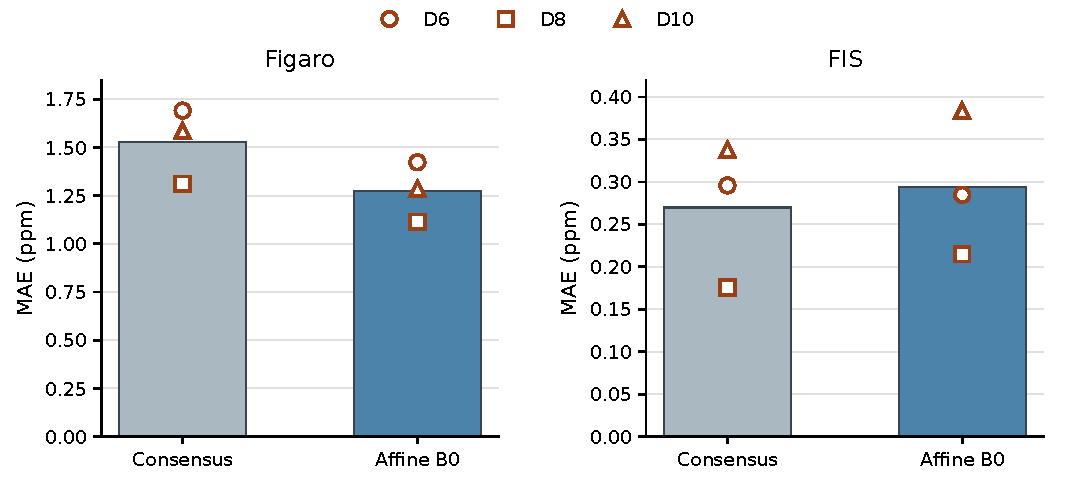
\includegraphics[width=.92\linewidth]{fig_1_historical_mae.pdf}
\caption{Development RF historical-only family MAE. Bars are equal-session means; outlined circles, squares and triangles show D6, D8 and D10, respectively. The Figaro and FIS panels use different vertical scales. Each family retains six correlated peer configurations on the same 100 exposures per session.}\label{fig:historical}\end{figure}
Table~\ref{tab:family} reports exact array-based family/session values. Figaro MAE improves on all three days. FIS MAE improves on D6 and worsens on D8/D10, although its strict exceedance count falls by two on each day. Endpoint directions therefore differ. The three affine lambdas have identical B0 predictions by construction and exact verification.
\begin{table}[H]\centering\small
\caption{Exact historical-only RF family/session values from prediction arrays; each cell has 100 exposures and 600 outputs. Counts are strict 1 ppm exceedances.}\label{tab:family}
\setlength{\tabcolsep}{4pt}\begin{tabular}{llrrrrr}
\toprule
Day & Family & Raw MAE & Affine MAE & $H$ MAE & Raw count & Affine count \\ \midrule
D6 & Figaro & 1.6909 & 1.4229 & -0.2680 & 366 & 298 \\
D6 & FIS & 0.2957 & 0.2847 & -0.0110 & 45 & 43 \\
D8 & Figaro & 1.3110 & 1.1139 & -0.1971 & 324 & 264 \\
D8 & FIS & 0.1757 & 0.2147 & 0.0390 & 39 & 37 \\
D10 & Figaro & 1.5850 & 1.2858 & -0.2992 & 366 & 309 \\
D10 & FIS & 0.3378 & 0.3836 & 0.0458 & 90 & 88 \\
\bottomrule\end{tabular}\end{table}

\FloatBarrier

\subsection{Additional references and forgetting}
Table~\ref{tab:incremental} compares B20 with each estimator's own B0, rather than attributing its historical advantage to new queries. All fifteen pooled RF B20 affine MAE changes are positive (adverse), although some lower-budget pooled point changes are favorable; the complete discrete-budget grid is retained. Under the envelope mask, changes are 0.0029, 0.0056 and 0.0115 ppm for $\lambda=1,.95,.90$. The native $.95$ comparator has MAE 0.7913 ppm and an incremental change 0.0070 ppm, with length-10 conditional bounds [0.0005, 0.0129] ppm. This tested coupled comparator does not improve pooled RF MAE. Exceedance directions, family effects and individual sessions differ; no universal statement about reference value follows.
\begin{table}[H]\centering\small
\caption{RF B20 changes from each affine estimator's common B0. Positive values worsen the endpoint. Conditional 95\% resampling bounds use block length 10. Last column counts sessions with a negative MAE change. All budgets, families and lengths are in the supplement.}\label{tab:incremental}
\setlength{\tabcolsep}{4pt}\begin{tabular}{llrrrrr}
\toprule
Estimator & Schedule & $I$ MAE & Conditional bounds & $I$ $P_1$ (pp) & Bounds (pp) & MAE $<0$ \\ \midrule
Affine $\lambda=1$ & Periodic & 0.0105 & [0.0072, 0.0142] & -0.11 & [-0.56, 0.28] & 0/3 \\
Affine $\lambda=1$ & Random & 0.0017 & [0.0006, 0.0030] & -0.09 & [-0.24, 0.06] & 0/3 \\
Affine $\lambda=1$ & Confidence & 0.0125 & [0.0081, 0.0178] & 0.03 & [-0.42, 0.42] & 0/3 \\
Affine $\lambda=1$ & Envelope & 0.0029 & [-0.0001, 0.0056] & 0.25 & [0.00, 0.53] & 0/3 \\
Affine $\lambda=1$ & Information & 0.0030 & [-0.0007, 0.0065] & 0.06 & [-0.19, 0.42] & 0/3 \\
Affine $\lambda=.95$ & Periodic & 0.0146 & [0.0102, 0.0191] & -0.19 & [-0.81, 0.33] & 0/3 \\
Affine $\lambda=.95$ & Random & 0.0024 & [0.0008, 0.0044] & -0.13 & [-0.33, 0.05] & 1/3 \\
Affine $\lambda=.95$ & Confidence & 0.0196 & [0.0123, 0.0283] & 0.25 & [-0.33, 0.83] & 0/3 \\
Affine $\lambda=.95$ & Envelope & 0.0056 & [-0.0001, 0.0109] & 0.19 & [-0.08, 0.56] & 0/3 \\
Affine $\lambda=.95$ & Information & 0.0070 & [0.0005, 0.0129] & 0.25 & [-0.19, 0.83] & 0/3 \\
Affine $\lambda=.90$ & Periodic & 0.0215 & [0.0146, 0.0278] & -0.14 & [-0.86, 0.50] & 0/3 \\
Affine $\lambda=.90$ & Random & 0.0042 & [0.0012, 0.0074] & -0.07 & [-0.38, 0.17] & 1/3 \\
Affine $\lambda=.90$ & Confidence & 0.0323 & [0.0193, 0.0473] & 0.28 & [-0.33, 0.89] & 0/3 \\
Affine $\lambda=.90$ & Envelope & 0.0115 & [0.0008, 0.0212] & 0.25 & [-0.39, 0.83] & 0/3 \\
Affine $\lambda=.90$ & Information & 0.0200 & [0.0056, 0.0337] & 0.78 & [-0.11, 1.81] & 0/3 \\
\bottomrule\end{tabular}\end{table}

\begin{figure}[H]\centering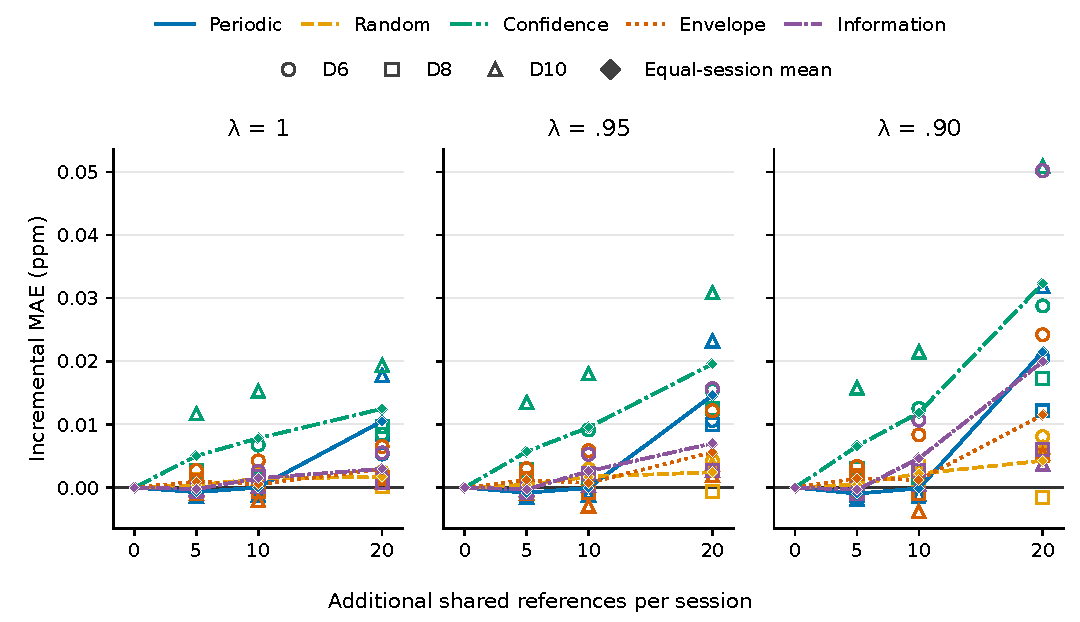
\includegraphics[width=\linewidth]{fig_2_affine_increment_mae.pdf}
\caption{Development RF pooled incremental MAE relative to each affine estimator's own B0, by update factor and schedule. Colors and line styles identify schedules; filled diamonds show equal-session means. Outlined circles, squares and triangles show D6, D8 and D10. All panels share one vertical scale; positive changes are adverse. Lines join evaluated discrete budgets only. Development-only conditional intervals and family values remain in the supplement.}\label{fig:incrementalmae}\end{figure}
\begin{figure}[H]\centering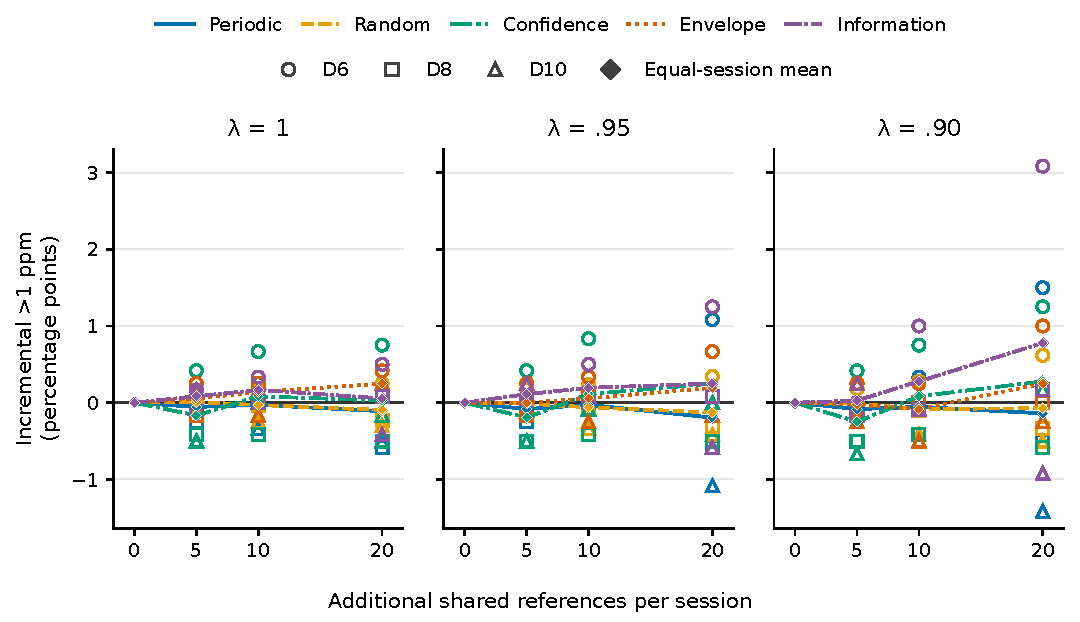
\includegraphics[width=\linewidth]{fig_3_affine_increment_exceedance.pdf}
\caption{Development incremental strict 1 ppm exceedance relative to own B0, in percentage points. Colors/line styles identify schedules, filled diamonds show equal-session means, and outlined circles/squares/triangles show D6/D8/D10. Panels share a vertical scale; positive changes are adverse. Lines join only evaluated budgets. MAE and exceedance can move in different directions.}\label{fig:incrementalp}\end{figure}
The cumulative envelope B20 estimate remains 0.7872 ppm and 29.11\% exceedance, compared with its own B0 at 0.7843 ppm and 28.86\%. Resampling intervals crossing zero are retained as conditional sensitivity bounds rather than interpreted as equivalence. Other schedules and block lengths, including unfavorable changes, remain visible.
\FloatBarrier

\subsection{Subset, support and upstream-model checks}
A concrete selection example is confidence B20 cumulative affine: unqueried MAE is 0.7403 ppm, but unchanged consensus on that same subset is 0.8580 ppm versus 0.8993 ppm on all exposures. The affine B0 MAE on those same unqueried exposures is 0.7243 ppm, so the positive-budget 0.7403 ppm is adverse against its own matched baseline. Selecting difficult exposures for purchase changes the unqueried population. Every subset now also has the estimator's own same-subset B0 and exact count, so subset selection and incremental prediction changes are distinguishable.

Concentration support and the 10\% relative tolerance are tabulated in Supplement S5 and the full numerical records. Both families have the same chamber-concentration support, while their errors differ. Reference-defined bands are evaluation diagnostics only.

A saved-input upstream-model sensitivity retains RF as primary. OLS historical affine MAE is 0.7678 ppm versus consensus 0.8652 ppm; ridge gives 0.9046 versus 1.0873 ppm. Under envelope B20, cumulative affine changes are $-0.0021$ and $-0.0025$ ppm for OLS and ridge. Native $.95$ changes are $-0.0037$ ppm for OLS and $+0.0039$ ppm for ridge. Thus the incremental pattern is model dependent. No model was refitted or promoted; OLS/ridge confidence uses peer MAD, unlike RF tree spread, and each model retains its own mask.

Paid queries in the last ten exposures and at exposure 100 are counted per run, then averaged over seeds and days (Supplement S6). Only exposure-100 purchases lack a subsequent scored prediction under reset; the other last-ten purchases can affect later outputs. All budgets remain charged.

\subsection{Containment is not assurance}\label{sec:boundresults}
Primary envelope-driven B20 midpoint width is 16.8528 ppm and containment 99.56\%, yet only 60 of 3,600 outputs (1.67\%) meet the conditional 1 ppm criterion. All 60 are unqueried: 60/2,880=2.08\%; queried outputs have none. No complete twelve-configuration unqueried exposure is assured under the original primary RF schedules. Sixteen primary B20 raw noncontainments occur without contradictions. Numerical consistency alone therefore does not establish containment.
\begin{table}[H]\centering\small
\caption{RF midpoint interval diagnostics on all exposures. Fractions average seeds within sessions and sessions equally; flags require a noncontradictory radius at most 1 ppm.}\label{tab:bounds}
\setlength{\tabcolsep}{4pt}\begin{tabular}{lrrrr}
\toprule
Schedule & $B$ & Width (ppm) & Contained (\%) & Flagged (\%) \\ \midrule
Historical only & 0 & 22.2412 & 99.78 & 0.61 \\
Periodic & 20 & 18.4844 & 99.50 & 1.28 \\
Random & 20 & 18.8071 & 99.50 & 1.19 \\
Confidence & 20 & 19.4958 & 99.28 & 0.78 \\
Envelope & 20 & 16.8528 & 99.56 & 1.67 \\
Information & 20 & 20.4082 & 99.72 & 1.28 \\
\bottomrule\end{tabular}\end{table}

The exact slope95/envelope B20 cross-tab reconciles 2,072 raw noncontainments: 749 contradictory outputs are contained by their descriptive hull, and 1,323 noncontradictory outputs remain outside their reported interval. This partition was checked by output identities. The complete 16-cell cross-tab, including zero cells and assurance, is in Supplement S7. Actual errors, rather than interval noncontainment alone, identify 503 false 1 ppm midpoint assurances among 2,287 assured outputs (21.99\%), and 503 among all 3,600 outputs (13.97\%). The 1,188 outside-and-assured entries are not themselves a false-assurance count. Primary midpoint bounds have 0/60 false assurances (0\%) and 0/3,600 overall, separately from their 16 noncontainments. The sensitivity remains a negative result. Broad primary bounds and failed narrower bounds are both retained.

The archived schedule grid contains repeated zero-budget runs that are numerically identical. After exact equality checks, the original grid reduces to one zero-budget run and 39 positive-budget masks per model/day/bound setting; the native schedules add 15 distinct runs across the evaluated models and days. These are computational identities on the same 300 physical development exposures, not additional experimental replication.

\section{Fixed-D10 temporal confirmation}\label{sec:c5}
\subsection{Frozen roles and complete execution}
A separately authorized temporal confirmation assessed D11, D12 and D13 using R1--R6 and R8--R13. The twelve frozen RF models were fitted only on D1, D2 and D4--D9, with the same seed 487, 100 trees, depth 5, minimum leaf size 5 and fit-only scaling. Initial correction calibration and scheduler normalization used D10 only. Every policy, budget, seed and assessment session reset independently to that same D10 state; no rolling recalibration or final-label carry occurred. R7/R14 and the UCI270 reservations remained excluded.

The complete predeclared comparison retained the two original primary contrasts, all five schedules, budgets 0/5/10/20, all random seeds 487--496, and the declared forgetting and fixed $.95$ information-controller extensions. Each current prediction, raw/reported interval and decision was persisted before purchase; a purchased reference affected later predictions only. All 129 replay paths and 12,900 pre-query records were committed before final performance summaries. A saved-output arithmetic audit reproduced all 40,635 per-run metric rows exactly, verified the fixed initial states and causal records, and checked unchanged source/model/development hashes. No integrity/access violation or numerical-update failure was found. The 300 exposures and 3,600 correlated outputs are separate from the development sample.

\subsection{Frozen benefit criterion and primary findings}
The criterion fixed before confirmation requires lower strict 1 ppm exceedance and nonpositive MAE change pooled and in both families. It applies separately to historical affine B0 versus unchanged consensus and to affine envelope B20 versus its own B0. Uniform-session improvement additionally requires no adverse session/family cell. The secondary schedule-superiority rule requires favorable exceedance and nonpositive MAE against periodic, random-seed mean and confidence, pooled and in both families (Section~\ref{sec:evaluation}).
Table~\ref{tab:c5primary} retains the pooled and both-family results. Historical affine correction reduces pooled MAE from 1.4570 to 1.3553 ppm and strict 1 ppm exceedance from 1,791/3,600 to 1,550/3,600 (49.75\% to 43.06\%). Figaro contributes 240 of the 241 net removed exceedances. FIS MAE instead increases from 0.8820 to 0.9471 ppm, worsening on all three sessions. Thus the frozen historical-benefit criterion requiring favorable exceedance and nonpositive MAE change in both families is not met; the finding is heterogeneous.

\begin{table}[H]\centering\small
\caption{Fixed-D10 temporal confirmation, distinct from development. MAE in ppm; counts are strict 1 ppm exceedances. B0 and envelope B20 use cumulative inverse affine correction. $N$ counts correlated configuration outputs, not independent exposures.}\label{tab:c5primary}
\setlength{\tabcolsep}{4pt}\begin{tabular}{lrrrrrrr}
\toprule
Scope & $N$ & Raw MAE & B0 MAE & B20 MAE & Raw count & B0 count & B20 count \\ \midrule
ALL & 3600 & 1.4570 & 1.3553 & 1.3257 & 1791 & 1550 & 1517 \\
Figaro & 1800 & 2.0320 & 1.7636 & 1.7481 & 1275 & 1035 & 1019 \\
FIS & 1800 & 0.8820 & 0.9471 & 0.9033 & 516 & 515 & 498 \\
\bottomrule\end{tabular}\end{table}


The original incremental comparison, cumulative affine envelope B20 against its own B0, reduces pooled MAE by 0.0297 ppm to 1.3257 ppm and exceedance by 33 outputs to 1,517/3,600 (42.14\%). Both family-aggregate MAE and exceedance changes are favorable, satisfying the prespecified descriptive incremental-benefit criterion. FIS improves relative to affine B0 (0.9471 to 0.9033 ppm), but its MAE remains worse than unchanged consensus (0.8820 ppm). This does not establish uniform improvement: pooled D12 MAE changes by +0.0049 ppm; Figaro/FIS D12 changes are +0.0071/+0.0027 ppm, and FIS D13 changes by +0.0068 ppm with one additional exceedance. Pooled D11/D13 MAE changes are $-0.0918/-0.0021$ ppm. All session/family numerators and denominators are in Supplement S10 and the full numerical files.

\begin{figure}[H]\centering
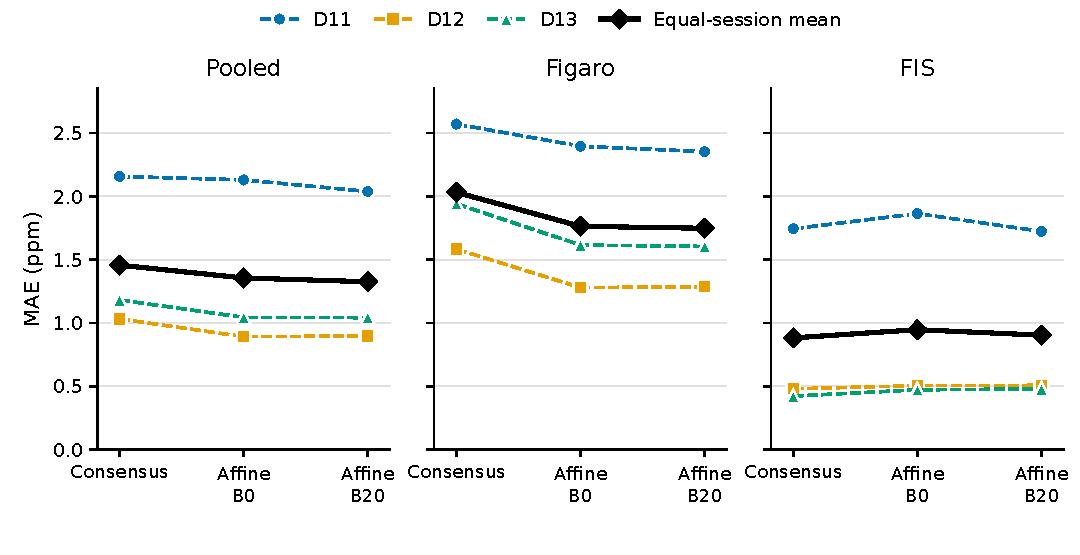
\includegraphics[width=\linewidth]{fig_4_c5_primary_mae.pdf}
\caption{Prespecified primary confirmation paths, with a shared vertical scale. D11 circles, D12 squares and D13 triangles show session MAE; black diamonds show equal-session means. Lines connect unchanged consensus, cumulative affine B0 and cumulative affine envelope B20, using the same frozen RF models and independent D10 resets. Each pooled session has 1,200 outputs and each family has 600 from 100 shared exposures. FIS B20 remains worse than consensus in aggregate; all session reversals remain visible.}\label{fig:c5mae}
\end{figure}

Fourteen of the fifteen pooled affine B20 MAE point changes are favorable in confirmation, whereas all fifteen were adverse in development. The confidence $.90$ change is adverse (+0.0047 ppm); confidence $\lambda=1$ improves MAE while worsening strict exceedance. The native $.95$ comparator changes pooled MAE by $-0.0551$ ppm, but remains an extension rather than a replacement primary. No method, factor, budget, family or seed was selected by its final outcome. Secondary envelope-schedule superiority is not established: against confidence at $\lambda=1$ B20, envelope has worse pooled MAE (+0.0078 ppm) and worse FIS MAE and exceedance.

\subsection{Scientific bound failures in a valid evaluation}
Table~\ref{tab:c5intervals} separates raw noncontainment, reported-set noncontainment, contradictions and actual midpoint false assurance. Envelope B20 has 284/3,600 raw noncontainments and 276/3,600 reported noncontainments, with eight contradictory outputs contained only by the descriptive hull. Mean width is 15.7129 ppm. Of 74 midpoint flags at 1 ppm, 38 are false: 38/74=51.35\% conditional and 38/3,600=1.06\% overall. Figaro contributes 1/1 false/assured and FIS 37/73. Queried outputs have 8/14 false/assured and 8/720 false/all; unqueried outputs have 30/60 and 30/2,880. These are midpoint-envelope diagnostics, not affine uncertainty intervals; RLS assurance remains unavailable.

\begin{table}[H]\centering\small
\caption{Primary envelope B20 interval diagnostics in confirmation. Outside counts use raw intersection and reported set separately. False/assured refers to actual midpoint error above 1 ppm among noncontradictory own-radius flags.}\label{tab:c5intervals}
\setlength{\tabcolsep}{4pt}\begin{tabular}{lrrrrrr}
\toprule
Scope & $N$ & Raw out & Report out & Contradictions & Width (ppm) & False/assured \\ \midrule
ALL & 3600 & 284 & 276 & 8 & 15.7129 & 38/74 \\
Figaro & 1800 & 56 & 56 & 0 & 25.4683 & 1/1 \\
FIS & 1800 & 228 & 220 & 8 & 5.9575 & 37/73 \\
\bottomrule\end{tabular}\end{table}


These failures reject an unconditional hard-bound claim and remain scored scientific outcomes. They do not invalidate the otherwise verified evaluation. No confirmation bootstrap, bound retuning, model refit, favorable-seed selection or experiment repeat was performed. This is later-session evidence on the same apparatus, not certified physical uncertainty, independent-array validation or a new algorithmic claim.

\section{Discussion}\label{sec:discussion}
The completed temporal confirmation changes the incremental finding while preserving the family qualification. Under the frozen pooled-and-both-family criterion, the original affine envelope 20-check comparison improves pooled MAE from 1.3553 to 1.3257 ppm and strict 1 ppm exceedance from 43.06\% to 42.14\%. Fourteen of fifteen pooled B20 affine MAE changes are favorable in confirmation, compared with fifteen adverse changes in development. The stages remain separate; this reversal neither removes the adverse development evidence nor selects a new final-data winner. Historical benefit remains heterogeneous. FIS improves from affine B0 at 0.9471 to 0.9033 ppm with the primary schedule but remains worse in MAE than unchanged consensus at 0.8820 ppm. D12 and FIS D13 reversals preclude uniform-session improvement, and the envelope-schedule superiority criterion is unsupported.
\subsection{Control initialization before assigning reference value}
Historical correction already improves pooled RF performance before a new reference is bought in both stages; confirmation additionally supports an incremental aggregate benefit. The reporting identity in Eq.~\eqref{eq:decomp} exposes this distinction separately for MAE and exceedance. Retaining family results prevents a pooled improvement from concealing adverse FIS MAE. Additional-reference and schedule comparisons must use identical exposure keys and an effective same-estimator B0.

\subsection{Update information and conditional sensitivity}
Cumulative RLS can absorb new references: its gain is nonzero for informative regressors. The response depends on leverage, innovation and historical information, not merely 100 versus 20 rows. Forgetting at purchases discounts old information and ridge; it does not forget during unqueried exposures. The fixed $.95$ comparator and $.90$ sensitivity, including one native schedule, increase the scope of this development comparison without supporting a claim that any tested method is optimal. Actual state changes and leverage are archived.

In development, every pooled RF B20 affine MAE point change is adverse, while some lower-budget pooled point changes are favorable and endpoint and family patterns vary. OLS/ridge provide some small favorable incremental changes, showing dependence on upstream prediction and mask. Conditional resampling bounds help describe the frozen development paths; crossing zero does not prove absence or equivalence, and excluding zero does not confer population significance after sequential development. Quarter-path, lag-one and trend diagnostics expose temporal structure rather than assume away nonstationarity. The stated relative reference-uncertainty percentage is not an independent Gaussian noise floor for a paired contrast using common labels.

\subsection{Prediction sets and measurement assurance}
Conditional minimax midpoint behavior is distinct from empirical MAE. Projection's non-worsening property requires the actual residual to lie within the assumed interval. Hull containment cannot rescue a contradictory intersection. Frequent containment, a narrow radius and complete-array service assurance are separate properties. Confirmation records 38 false midpoint assurances among 74 flagged outputs (51.35\%) and among 3,600 total outputs (1.06\%), separately from 284 raw and 276 reported-set noncontainments. These are midpoint-envelope diagnostics, not affine uncertainty intervals. Standard conformal methods provide a useful future comparison only under their own exchangeability or sequential assumptions \cite{angelopoulos2021}; neither descriptive envelopes nor ordinary split conformal offer unconditional protection against arbitrary drift.

Traceable co-calibration requires characterized references and uncertainty propagation \cite{gruber2023,jcgm100,jcgm200}. Multiple accesses to one generated-concentration system cannot identify a shared reference bias. The current analysis is a reference-relative algorithm comparison. The fixed-D10 temporal confirmation provides distinct later-session evidence: family heterogeneity persists historically, while the original incremental aggregate criterion is met despite session reversals (Section~\ref{sec:c5}).

\section{Limitations}\label{sec:limitations}
Both stages use one chamber and array: three development assessment sessions and three separate confirmation sessions, each with twelve overlapping peer configurations. Sequential extensions were informed by earlier development results; family emphasis, forgetting, native scheduling and conditional resampling are declared extensions rather than independent preregistration. Error is relative to released nominal CO with stated relative uncertainty below 5.5\%, without exposure-level reference-error covariance or hard bounds. Certified physical uncertainty, independent-array coverage and a causal drift diagnosis are not established. Acquisition latency and cost are simulated, and resets limit the horizon of late purchases. R7/R14 and the UCI270 reserved batches remain unused; D11--D13 are evaluated only in the separately authorized fixed-D10 confirmation.

The calibrated hardware union includes units omitted from individual peer configurations; strict unseen-unit or single-sensor deployment is a different estimand. Late-core summaries omit transient and washout behavior, and anonymous positions do not establish serial/lot provenance. Inverse regression and numerical rank do not identify forward physical parameters. Empirical slopes and fixed temporal/session allowances are unvalidated future bounds. Conditional resampling is development-only; no confirmation bootstrap was performed. Ordinary block resampling requires regularity that these adaptive chronological paths may not satisfy; the saved conditional intervals neither rerun adaptive trajectories nor propagate fitting or reference uncertainty. The finite comparison does not rank all possible online methods. Complete local per-output provenance is retained; a public reproducibility deposit is not yet available.

\section{Conclusion}
The completed fixed-D10 temporal confirmation supports the prespecified incremental aggregate benefit: pooled affine B0 MAE falls from 1.3553 to 1.3257 ppm under the envelope-driven 20-check schedule, and strict 1 ppm exceedance falls from 43.06\% to 42.14\%. The same frozen descriptive criterion is met in both family aggregates, but adverse D12 and FIS D13 cells preclude uniform-session improvement and envelope-schedule superiority remains unsupported. FIS MAE improves from 0.9471 to 0.9033 ppm relative to affine B0 while remaining worse than unchanged consensus at 0.8820 ppm. Historical benefit is therefore heterogeneous, not uniformly confirmed.

The confirmation result reverses the development B20 pattern. In development, historical affine correction reduces pooled RF MAE from 0.8993 to 0.7843 ppm and strict exceedance from 34.17\% to 28.86\%, but all fifteen affine B20 MAE changes are adverse. Lower-budget and OLS/ridge sensitivities differ; development-only conditional resampling does not establish equivalence or population coverage. No confirmation bootstrap was performed. Confirmation also retains 38 false midpoint assurances among 74 flagged outputs and 38 among 3,600 total outputs, separately from interval noncontainment. These are midpoint-envelope diagnostics, not affine uncertainty intervals.

The contribution is an information-matched evaluation of established calibration rules across development and temporal confirmation. Each estimator's historical baseline, incremental contrast, family/session results, exact pairing and reference cost must remain visible. Both stages use one apparatus; the results establish neither a new calibration algorithm, certified uncertainty nor independent-array generalization.

\section*{Data and code availability}
The original measurements are publicly available from the UCI Machine Learning Repository under DOI \href{https://doi.org/10.24432/C5S302}{10.24432/C5S302} \cite{uci487}. Reproducibility code, protocols, saved predictions, query masks, causal-access records, numerical evidence and table/figure build inputs are hosted at \url{https://github.com/asayghe1/CO-Sensor-Reference-Calibration}. The original raw UCI archive is obtained from UCI and is not redistributed in the repository. R7/R14 raw data and the UCI270 reserved batches are excluded.
\section*{Acknowledgment}
The publicly released measurements and their documentation were provided by Javier Burgu\'es through the UCI Machine Learning Repository. The associated experimental studies are acknowledged in Refs.~\cite{burgues2018linear,burgues2018opls}.
\section*{Declaration of generative AI and AI-assisted technologies in the writing process}
During preparation of this work, the authors used OpenAI ChatGPT and Codex to assist with software drafting and checking, analysis/reporting code, manuscript organization, exposition and literature checks. Scientific figures were generated from the saved numerical evidence; no generative image model was used to create or alter experimental results. The authors remain responsible for the content of the article.
\bibliographystyle{unsrtnat}
\bibliography{references}
\end{document}
